\documentclass[a4paper,12pt]{memoir}

\usepackage{amssymb,amsmath,amsthm}
\usepackage[latin1]{inputenc}
\usepackage{graphicx}
\usepackage{listings}

\newcommand{\ltwo}[2]{\int^1_0 #1 #2 dx}
\newcommand{\norme}[1]{\|#1\|_{E}}
\newcommand{\norml}[1]{\|#1\|_{L^2}}
\newcommand{\dx}[0]{\;dx}
\newcommand{\bp}[0]{\begin{pmatrix}}
\newcommand{\ep}[0]{\end{pmatrix}}
\newcommand{\omt}[0]{\Omega(t)}
\newcommand{\intom}[0]{\int\limits_{\Omega}}
\newcommand{\intpom}[0]{\int\limits_{\partial \Omega}}
\newcommand{\dom}[0]{\;d \Omega}
\newcommand{\intomt}[0]{\int\limits_{\omt}}
\newcommand{\intpomt}[0]{\int\limits_{\partial \omt}}
\newcommand{\domt}[0]{\;d \omt}
\newcommand{\ds}[0]{\;d S}
\newcommand{\drt}[1]{\frac{d #1}{dt}}
\newcommand{\pdrt}[1]{\frac{\partial #1}{\partial t}}
\newcommand{\be}[0]{\begin{equation}}
\newcommand{\ee}[0]{\end{equation}}
\newcommand{\lt}[2]{(#1,#2)_{\Omega}}
\newcommand{\ltp}[2]{(#1,#2)_{\partial \Omega}}

\usepackage{color}

\theoremstyle{plain}
\newtheorem{master}{}[chapter]
\newtheorem{definition}[master]{Definition}
 
\definecolor{dkgreen}{rgb}{0,0.6,0}
\definecolor{gray}{rgb}{0.5,0.5,0.5}
\definecolor{mauve}{rgb}{0.58,0,0.82}
\definecolor{backr}{RGB}{255,102,0}

 
\lstset{ %
  language=Python,                % the language of the code
  basicstyle=\footnotesize,           % the size of the fonts that are used for the code
  numbers=left,                   % where to put the line-numbers
  numberstyle=\tiny\color{gray},  % the style that is used for the line-numbers
  stepnumber=1,                   % the step between two line-numbers. If it's 1, each line 
                                  % will be numbered
  numbersep=5pt,                  % how far the line-numbers are from the code
  backgroundcolor=\color{white},      % choose the background color. You must add \usepackage{color}
  showspaces=false,               % show spaces adding particular underscores
  showstringspaces=false,         % underline spaces within strings
  showtabs=false,                 % show tabs within strings adding particular underscores
  frame=single,                   % adds a frame around the code
  rulecolor=\color{black},        % if not set, the frame-color may be changed on line-breaks within not-black text (e.g. commens (green here))
  tabsize=2,                      % sets default tabsize to 2 spaces
  captionpos=b,                   % sets the caption-position to bottom
  breaklines=true,                % sets automatic line breaking
  breakatwhitespace=false,        % sets if automatic breaks should only happen at whitespace
  title=\lstname,                   % show the filename of files included with \lstinputlisting;
                                  % also try caption instead of title
  keywordstyle=\color{blue},          % keyword style
  commentstyle=\color{dkgreen},       % comment style
  stringstyle=\color{mauve},         % string literal style
  escapeinside={\%*}{*)},            % if you want to add a comment within your code
  morekeywords={*,...}               % if you want to add more keywords to the set
}


\title{Womersley flow with POD computation}
\author{H�kon �sterb�}


\begin{document}
\maketitle

\section{Introduction and background}
In this project we will look at Womersley flow in a channel or a cylinder. We will the do a Proper Orthogonal Decomposition 
of the flow and investigate how good this decomposition is. 
\subsection{Navier-Stokes and Womersely flow}
First of all the Navier-Stokes equation can be written as
\begin{align}
    u_t + u\cdot \nabla u &= -\nabla p + 2\nu\nabla \cdot  \epsilon(u) + f\\
    \nabla \cdot u &= 0
\end{align}
if we set $\rho = 1$, where $\epsilon(u) = \frac{1}{2}(\nabla u + (\nabla u)^T))$.
We will use a channel or a cylinder as our domain $\Omega$ with radius $R$ and set $x$ as the direction along the channel/cylinder.
$x = 0$ will be the inlet of the flow, and $x = L$ will be the outlet.
The boundary $\partial \Omega$ will be decomposed into $\partial \Omega_W$ for the walls, $\partial \Omega_I$ for the inlet of the tube 
and $\partial \Omega_O$ for the outlet. 
For Womersley flow we impose that the velocity $u$ is in $x$ direction, only varying with the radius of the cylinder and that 
$\frac{\partial p}{\partial x}$ is a function of time. 
\begin{align}
    u &= \begin{pmatrix} w(r,t)\\0\\0\end{pmatrix}\\
    \frac{\partial p}{\partial x} &= q(t)
\end{align}
Further we impose the no-slip boundary condition on the walls for $u$ and Neumann conditions 
on the inlet and outlet. For the pressure we prescribe $p_1(t)$ for the inlet and $p_2(t)$ for the outlet and Neumann conditions on the walls.
Now our model of the flow looks like this:
\begin{align}
    u_t + u\cdot \nabla u &= -\nabla p + 2\nu\nabla \cdot  \epsilon(u) + f \label{nseq}\\
    \nabla \cdot u &= 0\\
    u|_{\Omega_W} &= 0 \\
    \nabla u n|_{\Omega_I \cup \Omega_O} &= 0\\
    \nabla p\cdot n|_{\Omega_W} &= 0\\
    p|_{\Omega_I} &= p_1(t) \\
    p|_{\Omega_O} &= p_2(t) 
\end{align}
%We see that the Womersley flow velocity trivialy is divergence free, and we can get a simplyfied verson of the NS-equation (\ref{nseq})
%\begin{equation}
\section{Incremental Pressure Correction Scheme}
To solve the Navier-Stokes equation we will use the Incremental Pressure Correction Scheme(IPCS).
We first solve for a tentative velocity, then compute a new velocity by correcting the pressure.

The discretization in time is done with Backwards Euler 
\be\pdrt{u}(t_{n+1}) \approx \frac{u^{n+1} - u^n}{\Delta t}.\ee
The Navier-Stokes equation is then
\begin{align}
    u^{n+1}  + \Delta t u^{n+1} \cdot \nabla u^{n+1} &= -\Delta t \nabla p^{n+1} + \Delta t 2\nu \nabla \cdot \epsilon(u^{n+1}) + f^{n+1}
    \\ \nabla \cdot u^{n+1} &= 0
\end{align}
The non-linearity $u^{n+1} \cdot \nabla u^{n+1}$ can be dealt with in several ways, but here we will linearize the term by 
$u^n \cdot \nabla u^{n+1}$. The equation then becomes
\be\label{nonlinns} u^{n+1}  + \Delta t u^{n} \cdot \nabla u^{n+1} = -\Delta t \nabla p^{n+1} + \Delta t 2\nu \nabla \cdot \epsilon(u^{n+1}) + f^{n+1}\ee
The tentative velocity is calculated by evaluating $\nabla p$ as the previous computed value, 
and neglecting the incompressibility condition. 
It will be denoted by $u^*$ 
\be\label{nonlinnst} u^*  + \Delta t u^n \cdot \nabla u^* = -\Delta t \nabla p^n + \Delta t 2\nu \nabla \cdot \epsilon(u^*)+f^{n+1}.\ee
This is linear and solvable. Let $u^s = u^{n+1} - u^*$. Then subtracting equation (\ref{nonlinnst}) from (\ref{nonlinns}) we get
\begin{align}
    u^s + q(u^s) &= -\Delta t\nabla \phi \label{useq1}
   \\ \nabla \cdot u^s &= - \nabla \cdot u^* \label{useq2}
\end{align}
where $q(u^s) = \Delta t (u^n \cdot \nabla u^s - 2\nu \nabla \epsilon(u^s))$ and $\phi = p^{n+1} - p^n$. Neglegting the $q$ term from the equation
and multiplying (\ref{useq1}) with $\nabla$ and using (\ref{useq2})
\be\label{phieq} \Delta t\Delta \phi = \nabla \cdot u^* \ee
one gets a poisson problem for $\phi$. After solving this mixed system one can update the new velocity and pressure explisitly
\begin{align}
    u^{n+1} &= u^* - \Delta t \nabla \phi \label{updateu}\\
    p^{n+1} &= \phi - p^n.\label{updatep}
\end{align}

\subsection{The weak form of IPCS}
The IPCS can now be transformed into a weak form.
We use the notation 
\begin{align}
    (a,b)_{\Omega} &= \intom ab \dx \mbox{ for scalars $a$, $b$}\\
    (u,v)_{\Omega} &= \intom u\cdot v \dx\mbox{ for vectors $u$, $v$}\\
    (A,B)_{\Omega} &= \intom A:B \dx\mbox{ for matrices $A$, $B$} \\
    (u,v)_{\partial \Omega} &= \intpom u\cdot v\ds\mbox{ for vectors $u$, $v$}\\
\end{align}
The equation for the tentative velocity is
\be\label{tent} u^*  + \Delta t u^n \cdot \nabla u^* = -\Delta t \nabla p^n + \Delta t 2\nu \nabla \cdot \epsilon(u^*) + u^n + f^{n+1}.\ee
Multiplying with a testfunction $v$ and integrating over the domain $\Omega$ gives
\be \lt{u^*}{v} + \Delta t \lt{u^n\cdot \nabla u^*}{v} - \Delta t 2\nu \lt{\nabla \cdot \epsilon(u^*)}{v}= 
-\Delta t\lt{\nabla p^n}{v} + \lt{u^n}{v} + \lt{f^{n+1}}{v}. \ee
Let $a_1(u^*,v)$ be the right hand side and $L_1(v)$ be the left hand side.
Doing an integration by parts gives
\begin{align}
    \lt{\nabla \cdot \epsilon(u^*)}{v}&=  \intom (\nabla \cdot \epsilon(u^*))\cdot v\dx\\
                                      &= - \intom \epsilon(u^*) : \nabla v\dx + \intpom \epsilon(u^*)n \cdot v\ds \\
                                      &= - \intom \epsilon(u^*) : \nabla v\dx + \frac{1}{2}\intpom \nabla u^* n \cdot v \ds + 
    \frac{1}{2}\intpom (\nabla u^*)^T n\cdot v \ds \label{epsipb}\\ 
\end{align}
The test function $v$ is defined such that $v$ is zero on the part of the boundary where Dirichlet boundary condition are imposed.
Hence the term $\nabla u^*n \cdot v$ is equal to zero on the whole boundary.
Using this and (\ref{epsipb}), $a_1(u^*,v)$ becomes
\be a_1(u^*,v) = \lt{u^*}{v} + \Delta t \lt{u^n\cdot \nabla u^*}{v} + \Delta t 2 \nu \lt{\epsilon(u^*)}{\nabla v} - \Delta t \nu \ltp{(\nabla u^*)^T n}{v}\ee 
For $L_1$ we get
\begin{align} 
    L_1(v) &= -\Delta t\lt{\nabla p^n}{v} + \lt{u^n}{v} + \lt{f^{n+1}}{v}\\
           &= \Delta t(\lt{p^n}{\nabla \cdot v} - \ltp{p^n v}{n}) + \lt{u^n}{v}+ \lt{f^{n+1}}{v}
\end{align}

Multiplying the pressure equation with a test function $q$ and integrating gives
\be \lt{\Delta \phi}{q} =\frac{1}{\Delta t} \lt{\nabla \cdot u^*}{q} \ee
Integration by parts of the Laplace term gives
\begin{align}
    \lt{\Delta \phi}{q} &= -\lt{\nabla \phi}{\nabla q} + \ltp{\nabla \phi}{qn}\\
                        &= -\lt{\nabla \phi}{\nabla q} + \ltp{\nabla u^s}{qn}
\end{align}
From the definition of $u^s$ we have that $u^s|_{\Omega_W} = 0$. We have Dirichlet conditions on $\Omega_I \cup \Omega_O$ hence 
$q|_{\Omega_I \cup \Omega_O} = 0$. This imply that $\ltp{\nabla u^s}{qn} = 0$.
In Fenics this can be written as
\begin{lstlisting}
# Tentative velocity step
F1 = inner(u,v)*dx + k*inner(grad(u)*u0,v)*dx \
    + k*2*nu*inner(epsilon(u),grad(v))*dx\
    - k*nu*inner(grad(u).T*n,v)*ds \
    -k*inner(p0,div(v))*dx + k*inner(p0*v,n)*ds \
    - inner(u0,v)*dx - k*inner(f,v)*dx
a1 = lhs(F1)
L1 = rhs(F1)

# Pressure correction
a2 = inner(grad(q), grad(p))*dx
L2 = inner(grad(q), grad(p0))*dx - (1/k)*q*div(u1)*dx

# Velocity correction
a3 = inner(v, u)*dx
L3 = inner(v, u1)*dx - k*inner(v, grad(p1 - p0))*dx
\end{lstlisting}

\section{Verification of solver}
The Womersley flow has an analytical solution but this involves besselfunctions with complex 
arguments, and I failed to find an implementation of these in any python library.
Instead we will verify our solver by using a manufactured solution on the 2D channel domain.
Setting $u = (v(y,t),0)$ where $v(y,t)= Ae^{at}sin(\pi n y/R)$ we get a divergens free solution
with $u|_{\Omega_W} = 0$. We can now calculate $f(t,x,y)$ by inserting $u$ in the Navier-Stokes equation
\begin{align}
    f_x &= v_t + \frac{\partial p}{\partial x} - \nu v_{yy}\\
    &= (a+\frac{\nu \pi^2 n^2}{R^2})Ae^{at}\sin(\pi n y/R) + \frac{\partial p}{\partial x}\\
\end{align}
Setting $p(x,y,t) = -sin(8\pi t/T)x$, where $T$ is the end time, gives us $4$ cycles of the sinus function.

Since we use linear elements in space and linear discretization in time we should expect that 
the error to linearly decrees with $\Delta t$ and $h$, where $h$ is the height of the triangles in the mesh.
Increasing the number of triangles in the mesh will decrees $h$ so we can write  
\begin{equation}
    E = O(\Delta t) + O(\frac{1}{N})
\end{equation}
where $N$ is the number of triangles. If we set $E_i$ to the error where we have used $N = D2^{i+1}$ and 
$\Delta t = 2^{-(i+1)}$ we should have approximately $E_i 2^i = C$ where $C,D$ are constants.
Form figure (\ref{fig:error}) we see this relationship.
\begin{figure}[htb]
\centering
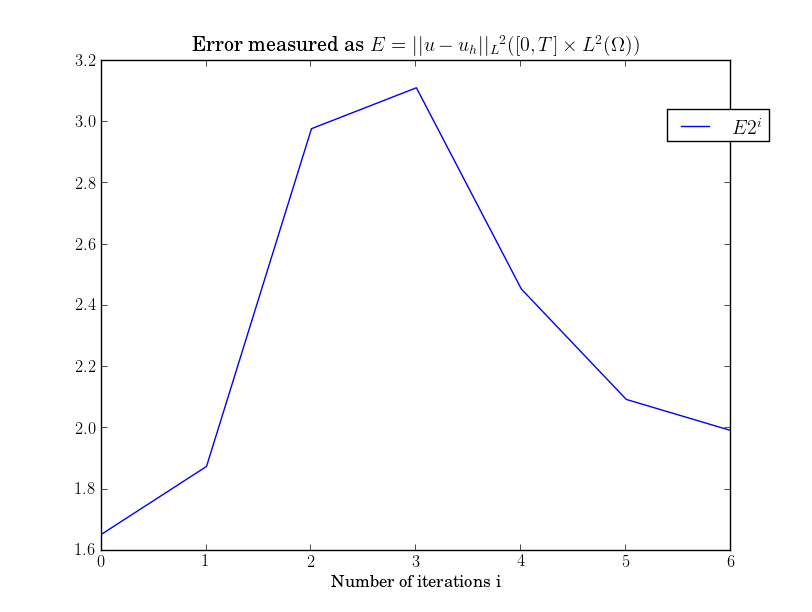
\includegraphics[width=0.8\textwidth]{error.png}
\caption{Error divided by step}
\label{fig:error}
\end{figure}

\section{Proper Orthogonal Decomposition}
The idea here is to find the best basis for describing our velocity field $u(x,t)\in [0,T]\times V$. By the best basis 
we mean that for all $k$ and given an inner product $||.||$ we want to find a set of functions $\phi_i$ and $a_i$ 
such that
\begin{equation}
    \min ||u - \sum_{i=1}^k a_i(t) \phi_i(x)||
\end{equation}
The decomposition can be computed in spacial or time domain. In CFD we often have large amount of spacial points, 
and few time points. Hence we will do less work by decomposing in time. Here we will only describe the time decomposition.
To calculate $a_i$ we have to solve the eigenvalue problem
\begin{equation}
    \frac{1}{T} \int\limits_0^T C(m,n) a_i(n) \; dn = \lambda_i a_i(m)
\end{equation}
for $C_{mn} = (u(x,m), u(x,n))_{\Omega}$. The coefficients are scaled according to 
\begin{equation}
    \frac{1}{T} \int\limits_0^T a_i(t) a_j(t) \; dt = \lambda_i \delta_{ij}
\end{equation}
Now we compute the basis by
\begin{equation}
    \phi_i = \frac{1}{\lambda_i T} \int\limits_0^T a_i(t) u(x,t) \; dt
\end{equation}
In our case we only have the velocity field in discrete time points $u^m = u(x,t_m)$.
So the integration will be the average of the sum instead.

This can be implemented in Fenics by (here we compute the basis for the fluctuating flow only):
\begin{lstlisting}
us = self.us 
V = us[0].function_space()
M = len(us)

# Compute mean velocity
u_0 = Function(V)
for u in us:
    u_0.vector()[:] += u.vector()
u_0.vector()[:] = 1./M*u_0.vector()

# Compute varying velocity
um = []
for u in us:
    um_i = u.copy(True)
    um_i.vector()[:] -= u_0.vector()
    um.append(um_i)
print "Mean and varying velocity computed" 

# Compute correlation matrix
C = np.zeros([M,M])
for n in range(M):
    for m in range(n+1):
        C[n,m] = (1./M)*assemble(inner(um[n],um[m])*dx)
        C[m,n] = C[n,m]
print "Correlation matrix computed"

# Compute eigenvalues
eigval, eigvec = np.linalg.eig(C)

# Remove complex values due to roundoff errors
eigval = eigval.real
eigvec = eigvec.real

# Scale eigenvectors
A = self.A
for i in range(M):
    if eigval[i] > 10e-16:
        print eigval[i]
        A.append(np.sqrt(eigval[i]*M)*eigvec[:,i])
    else : 
        break;

# Assure that order of POD is ok.
if k > len(A):
    k = len(A)
print "Eigenvalues/vectors computed and scaled"

# Basis velocity
ub = self.ub
for i in range(k):
    phi_i = Function(V)
    for m in range(M):
        phi_i.vector()[:] += A[i][m]*um[m].vector()
    phi_i.vector()[:] = 1./(M*eigval[i])*phi_i.vector()
    ub.append(phi_i)
print "Basis computed"
\end{lstlisting}

\subsection{POD error analysis}
We can do numerical experiments to check how good the POD is. This is done here by 
letting $E_k$ be the error in a $k$ order POD
\begin{equation}
    E_k = ||u_h - \sum_{i=1}^k a_i \phi_i||_{L^2([0,T]\times L^2(\Omega))}.
\end{equation}
Figure (\ref{fig:pod2d}) and (\ref{fig:pod3d}) show that the error goes fast to zero. We also see that in 3D the POD 
needs higher order than in 2D.

\begin{figure}[htb]
\centering
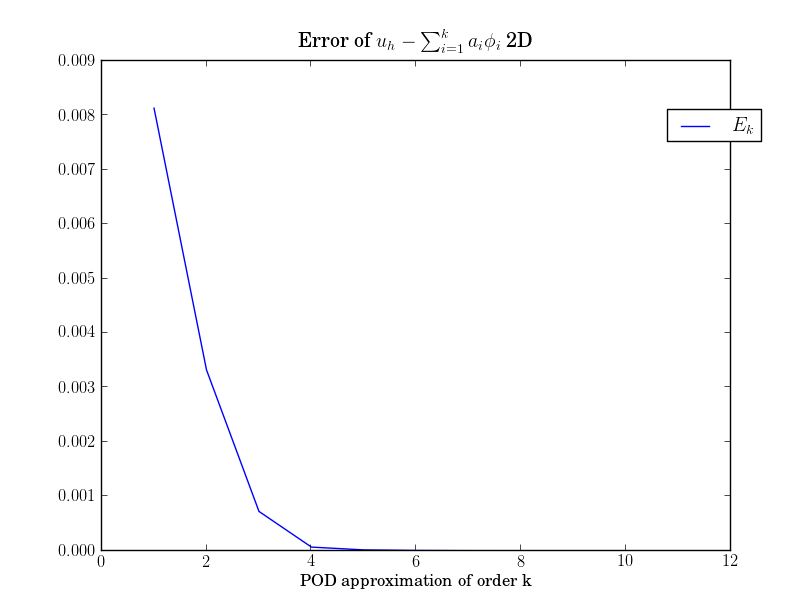
\includegraphics[width=0.8\textwidth]{poderror2d.png}
\caption{Error of POD order, 2D}
\label{fig:pod2d}
\end{figure}

\begin{figure}[htb]
\centering
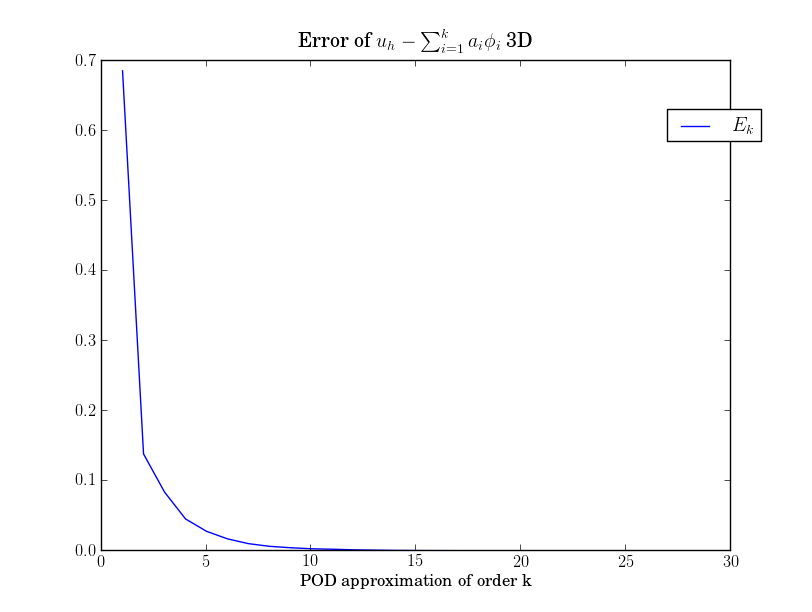
\includegraphics[width=0.8\textwidth]{poderror3d.png}
\caption{Error of POD order, 3D}
\label{fig:pod3d}
\end{figure}

\end{document}
